\def\baselinestretch{1}
\section{Descrizione algoritmo}
\def\baselinestretch{1.66}
\thispagestyle{headings}
\subsection{Pseudo codice}

\textbf{L'insertimento} nella struttura dati creata va effettuare prima una ricerca
del nodo di chiave $key1$. Se dovesse riscontrare un esito negativo si procede
alla allocazione di un hashtable e un nuovo nodo. In caso contrario si procede alla ricerca
di una cella della tavola di hash con la $key2$, se anche questa ricerca restituisce un esito
negativo allora si procede con l'inserimento.

\BlankLine
\IncMargin{1.5em}
\begin{algorithm}[H]
\setstretch{1.1}
\caption{Insert}
\SetKwData{Left}{left}\SetKwData{This}{this}\SetKwData{Up}{up}
\SetKwFunction{Union}{Union}\SetKwFunction{FindCompress}{FindCompress}
\SetKwInOut{Input}{input}\SetKwInOut{Result}{result}
\SetKwIF{If}{ElseIf}{Else}{if}{:}{elif}{else:}{}
\Input{ key1, key2, string }
\Result{ $true$ if successfull, $false$ if not }
\emph{$node$ = Search in Red Black with $key1$}\;
\If{$\nexists \ node$} {
    \emph{new Hashtable()}\;
    \emph{new Node()}\;
    \emph{Hashtable.insert(key2, string)}\;
    \emph{Node.insert(key1, Hashtable)}\;
    return \emph{true}\;
}
\Else{\If{$\nexists \ node.Hashtable.search(key2)$} {
        \emph{node.Hashtable.insert(key2, d)}\;
        return \emph{true}\; }}
return \emph{false}\;
\end{algorithm}

\indent La \textbf{ricerca} controlla la correttezza delle chiavi e della stringa inserita nella tupla:
in caso di riscontro positivo la function ritorner\`a il nodo dell'albero. Questo comportamento \`e stato previsto
per poter evitare di effettuare una o pi\`u ricerche nella
procedura di cancellazione.

\BlankLine
\IncMargin{1.5em}
\begin{algorithm}[H]
\setstretch{1.1}
\caption{Search (retrieve) }
\SetKwData{Left}{left}\SetKwData{This}{this}\SetKwData{Up}{up}
\SetKwFunction{Union}{Union}\SetKwFunction{FindCompress}{FindCompress}
\SetKwInOut{Input}{input}\SetKwInOut{Result}{result}
\SetKwIF{If}{ElseIf}{Else}{if}{:}{elif}{else:}{}
\Input{ key1, key2, string }
\Result{node if found $or$ NIL if not found}
\emph{$node$ = Search in Red Black with $key1$}\;
\If{$\exists \ node$} {
    \emph{$data$ = node.Hashtable.search(key2)}\;
    \If{string = data } {
        return \emph{node}\;
    }
}
return \emph{NIL}\;
\end{algorithm}
\newpage
\indent La \textbf{cancellazione} di una tupla effettua una operazione di ricerca nella struttura dati.
Se la ricerca ha risconto positivo allora si procede con i due casi della rimozione:
se la chiave secondaria indicizza una hashtable in cui vi \`e presente un solo elemento, allora
si canceller\`a l'intero nodo red black, altrimenti si procede alla normale rimozione dalla hashtable.
\BlankLine
\IncMargin{1.5em}
\begin{algorithm}[H]
\setstretch{1.1}
\caption{Remove (delete)}
\SetKwData{Left}{left}\SetKwData{This}{this}\SetKwData{Up}{up}
\SetKwFunction{Union}{Union}\SetKwFunction{FindCompress}{FindCompress}
\SetKwInOut{Input}{input}\SetKwInOut{Result}{result}
\SetKwIF{If}{ElseIf}{Else}{if}{:}{elif}{else:}{}
\Input{ key1, key2, string }
\Result{true if deleted $or$ false if not}
\emph{node = Search in Red Black Hash}\;
\If{$node \neq NIL$} {
    \eIf{node.Hashtable.capacity = 1} {
    \emph{delete node}\;}
    {node.Hashtable.remove(key2)\;}
    return \emph{true}\;}
return \emph{false}\;
\end{algorithm}

\subsection{Diagrammi delle classe e dettagli architetturali}
\subsubsection{Nodi Binari}
\indent I nodi facenti parti degli alberi
binari sono nodi che derivano da una classe astratta che a sua
volta estende un nodo generico.\newline
\indent Per permettere agli alberi binari di usare come parametro
templato un generico nodo, si \`e sfruttato un particolare
pattern strutturale chiamato \textbf{CRTP} \textit{(Curiously recurring 
template pattern)}: una classe (e.g. ConcreteBinaryNode) eredita
da una classe astratta che usa il CRTP (e.g. AbstractBinaryNode ha come parametro templato un generico nodo), usando
come parametro di specializzazione se stessa. Il nodo concreto
RedBlack in pi\`u implementa la classe color. Si \`e scelta tale tecnica che non porta
miglioramenti sostanziali al codice se non quella di nascondere
dettagli implementativi e un' indipendenza dalla rappresentazione in memoria del colore.
\begin{center}
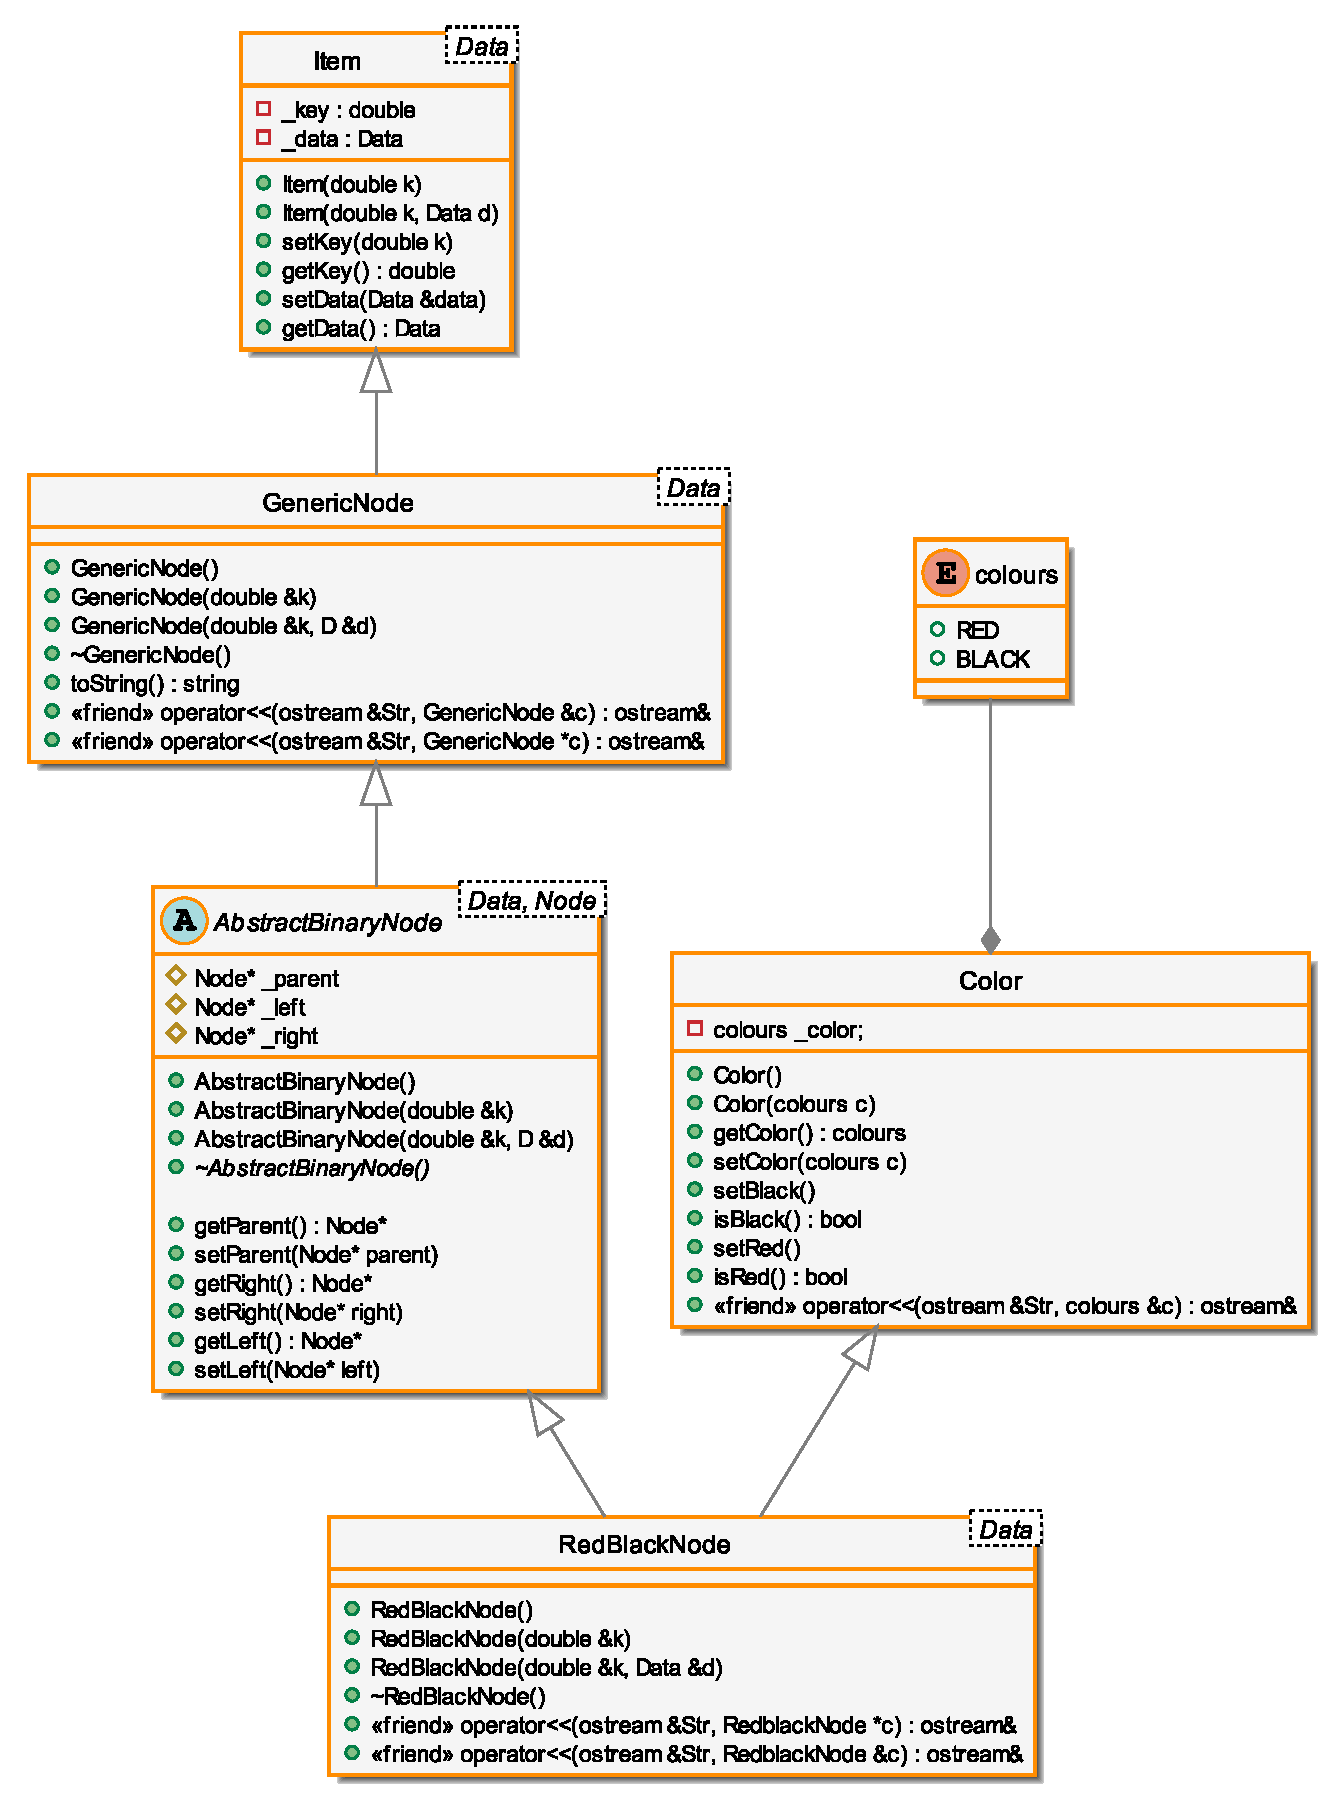
\includegraphics[scale=0.6]{src/rbhash/2img/nodes.eps}
\captionof{figure}{Nodi degli alberi}
\end{center}
\subsubsection{Alberi}
Un albero Rosso Nero \`e un albero binario di ricerca auto
bilanciante, per tanto si \`e scelto di estendere la classe
BinarySearchTree ed aggiungere i metodi di supporto al bilanciamento. Inoltre due metodi virtuali (insert e delete), sono
stati ridefiniti nell'implementazione del Red Black.
\textit{$insertNode()$} nella class RedBlackTree richiama tramite scope la insert
di BinarySearchTree e successivamente applica il
\textbf{fix} dei red black.
\begin{center}
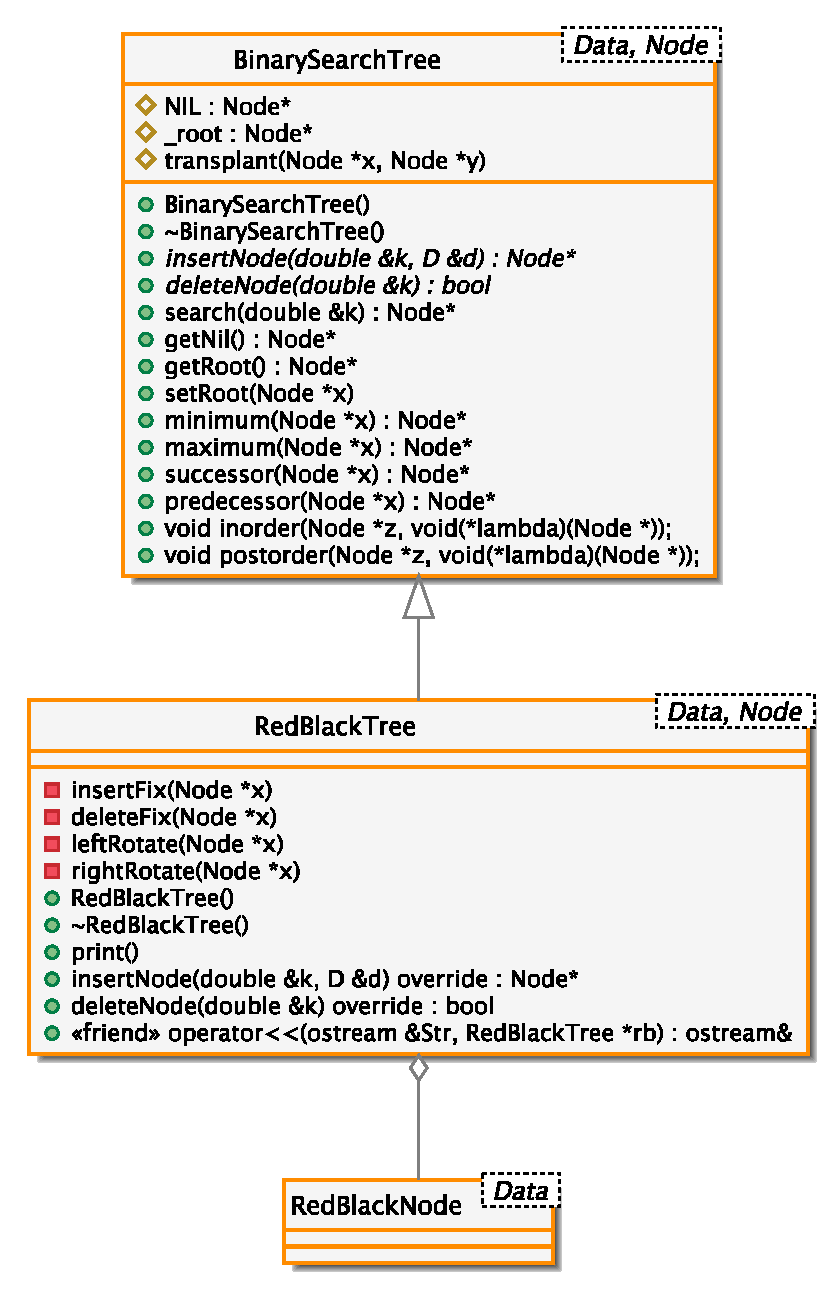
\includegraphics[scale=0.7]{src/rbhash/2img/trees.eps}
\captionof{figure}{Alberi}
\end{center}
\subsection{Hash Table}
Onde evitare di dover riscrivere codice si \`e scelto di sfruttare
il nodo generico anche per l'\textbf{HashTable}. A tal proposito
si \`e sviluppato una tabella hash ad \textbf{indirizzamento aperto} che
prende in input come paramentro templato, il dato da conservare.
Per risolvere le collisioni si \`e scelto di usare due funzioni hash:
\texttt{k} \`e un valore double che indica
la chiave, $\texttt{i}$ \`e l'iteratore che al massimo 
$\texttt{m}$ volte \footnote{m \`e il size dell'hashtable}  
applicher\`a la funzione di hash. La prima restituisce un indice con valore compreso
tra $[0, m]$, mentre la seconda funzione di hash un valore compreso tra $[1, m-1]$. 
Verr\`a usata la prima funzione di hash e in caso di collisione
si riapplicher\`a
$h(i, m) = (h_1(k) + i * h_2(k)) \ mod \ m$. Sebbene con un costo 
computazionale pi\`u alto, il doppio hashing risolve le collisioni
pi\`u in fretta rispetto allispezione lineare o quadratica.\newline \indent 
La funzione $search()$ nella class \textbf{HashTable}
\`e stata sovraccaricata per restituire valori diversi. Con la 
ricerca per valore si restituise, se disponibile un indice che 
usato nella seconda funzione di ricerca restituisce il dato.

\begin{center}
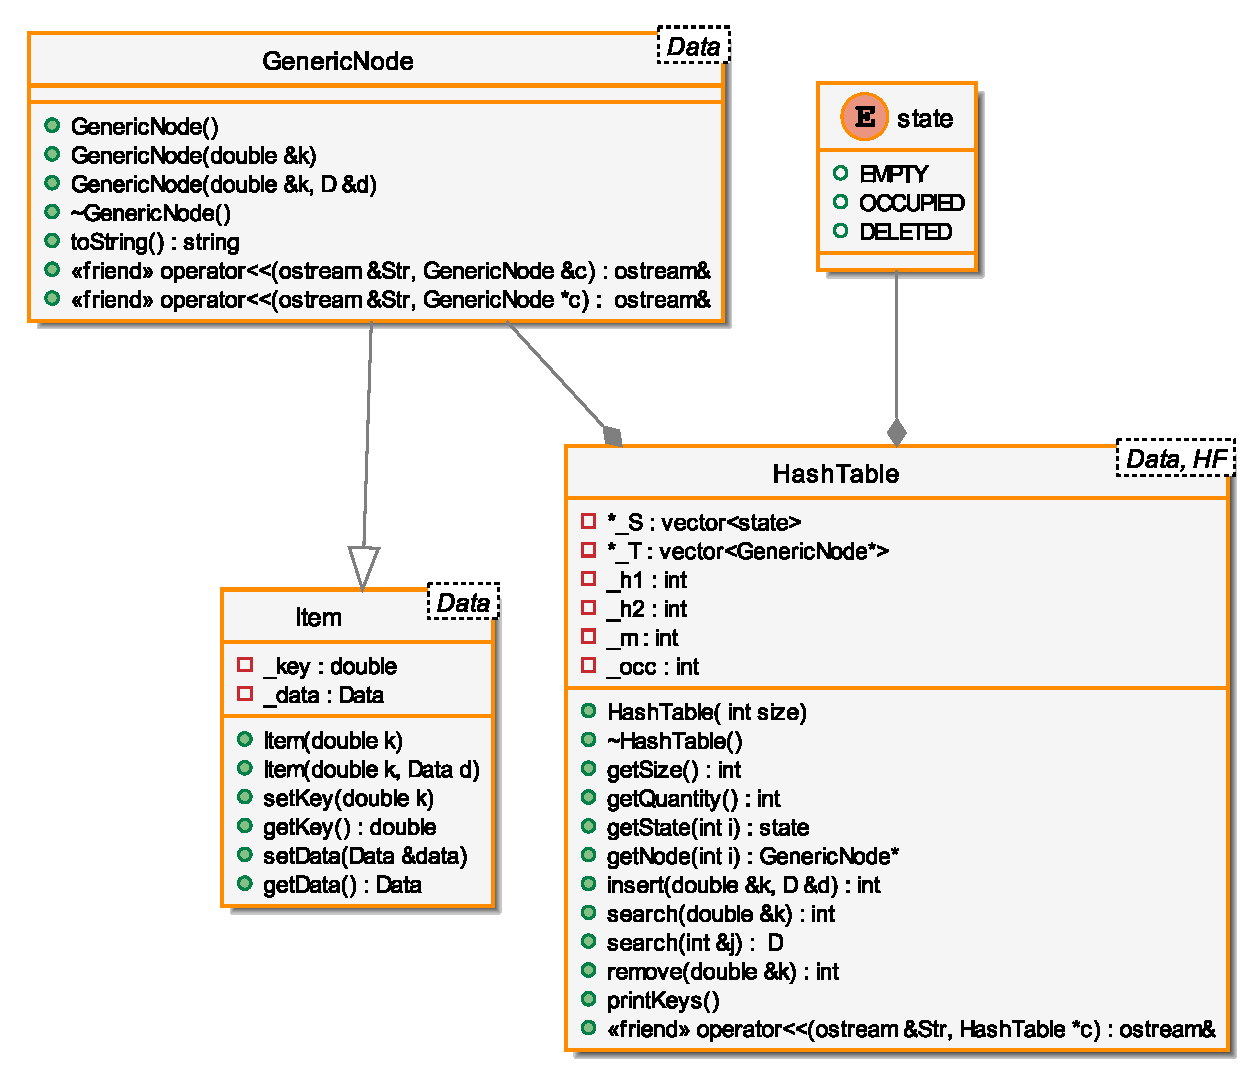
\includegraphics[scale=0.7]{src/rbhash/2img/hash.eps}
\captionof{figure}{Hash Table}
\end{center}

\newpage
\subsection{Red Black Hash}
La struttura dati realizzata fa uso degli alberi red black
e delle tavole di hash come spiegato nel primo paragrafo.
Si è scelto di usare una classe \textbf{Parser} per riempire la
struttura dati delle tuple contenute nel file di testo
o di quelle inserite tramite riga di comando.
\begin{center}
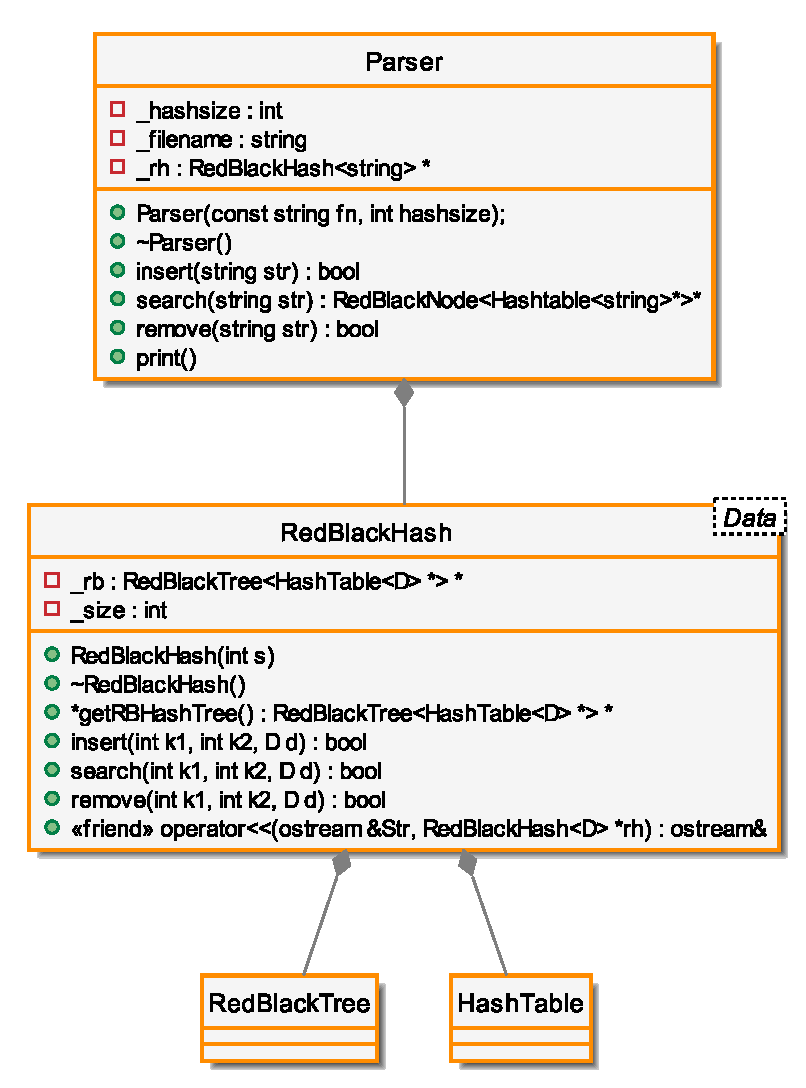
\includegraphics[scale=0.8]{src/rbhash/2img/rbhash.eps}
\captionof{figure}{Parser e RBH}
\end{center}